\documentclass[11pt]{article}
\usepackage[margin=20mm]{geometry}
\usepackage{amsmath}
\usepackage{float}
\usepackage{subfig}
\usepackage{listings,color,enumitem}
\definecolor{mygreen}{RGB}{28,172,0} % color values Red, Green, Blue
\definecolor{mylilas}{RGB}{170,55,241}
\usepackage{graphicx}

%\graphicspath{results/}
\title{Homework 2\\ \vspace{2mm}\Large{16-720A Computer Vision }}
\author{Matthew Swenson}

\begin{document}
	\maketitle
	
\section*{Q 1.5}
\begin{figure}[H]
\centering
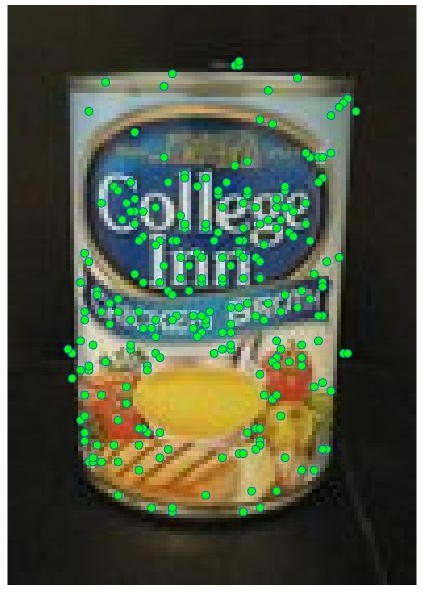
\includegraphics[width=.5\textwidth]{results/keypoints.jpg}
\caption{Using the difference of gaussians local extrema with intensity and principal 
curvature thresholding to determine points of interest. }
\end{figure}
\section*{Q 2.4}
Using a randomly distributed test pattern, my \texttt{testMatch} function produces the following 
results:
\begin{figure}[H]
\centering
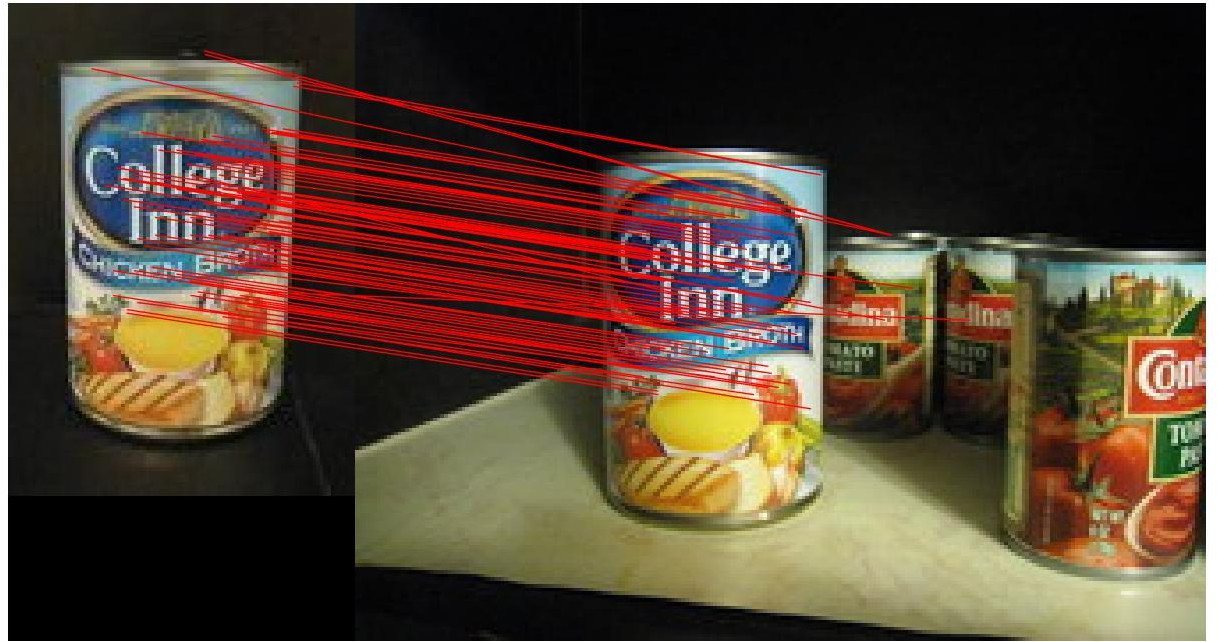
\includegraphics[width=.5\textwidth]{results/BRIEF_chickenbroth.jpg}
\caption{Comparison of model\_chickbroth.jpg and chickenbroth\_01.jpg}
\end{figure}
\begin{figure}[H]
\centering
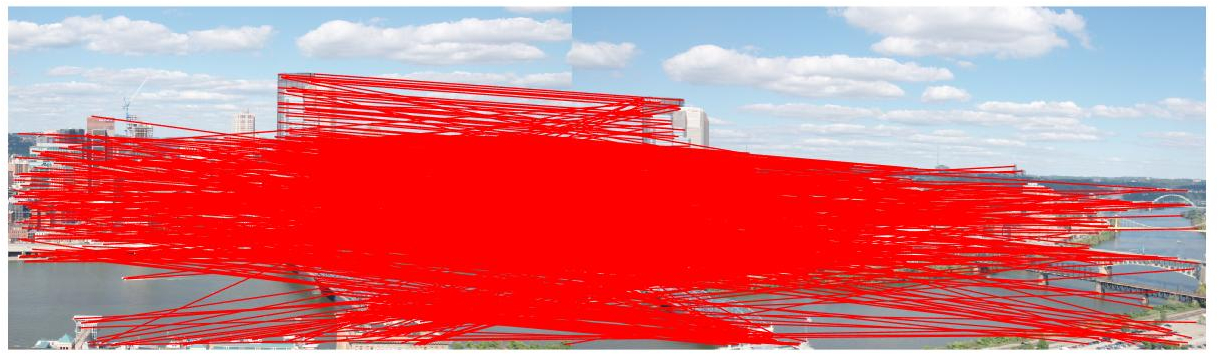
\includegraphics[width=\textwidth]{results/BRIEF_incline.jpg}
\caption{Comparison of the two incline images. There are over a thousand
matches, which generally obscures the photo. }
\end{figure}


The following are images of the black and white vertically oriented textbook cover matched with 
the textbook in various situations and orientations. In general, the matching performed worse when
the textbook being matched was at a different rotation from the black and white image. 
\begin{figure}[H]
    \begin{tabular}{cc}
        \subfloat[]{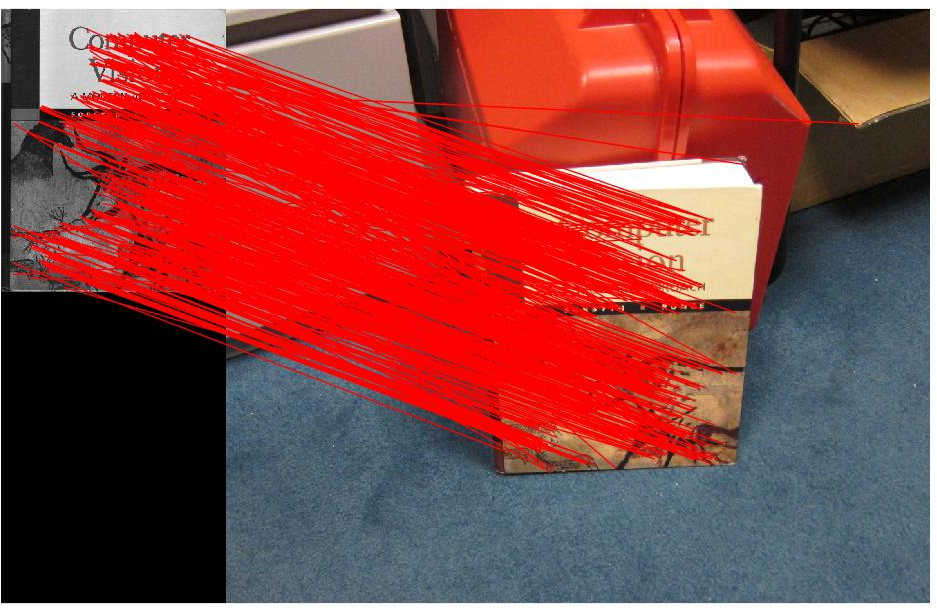
\includegraphics[width=.5\textwidth]{results/BRIEF_pfscan_stand.jpg}} &
        \subfloat[]{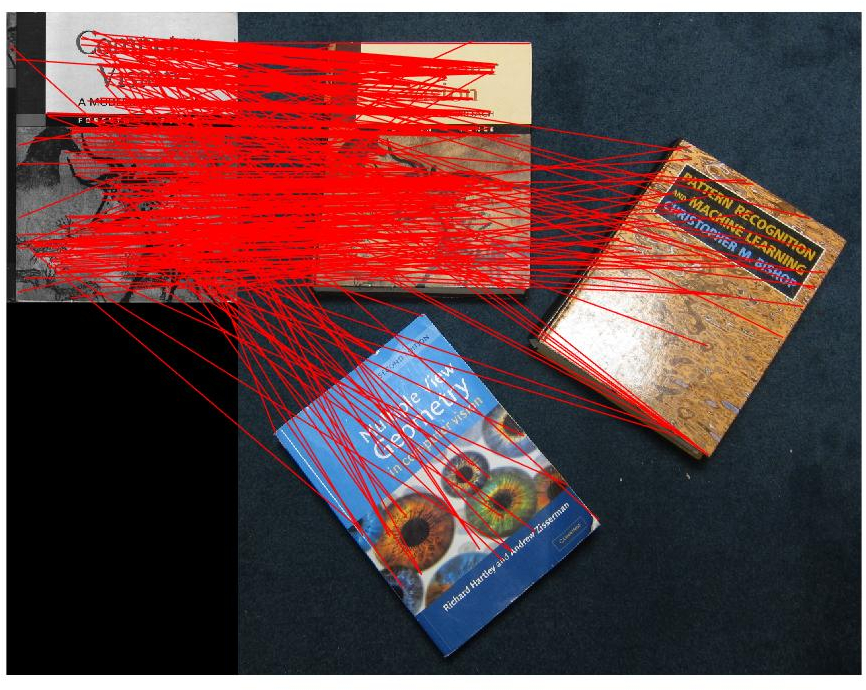
\includegraphics[width=.5\textwidth]{results/BRIEF_pfscan_floor.jpg}} \\
        \subfloat[]{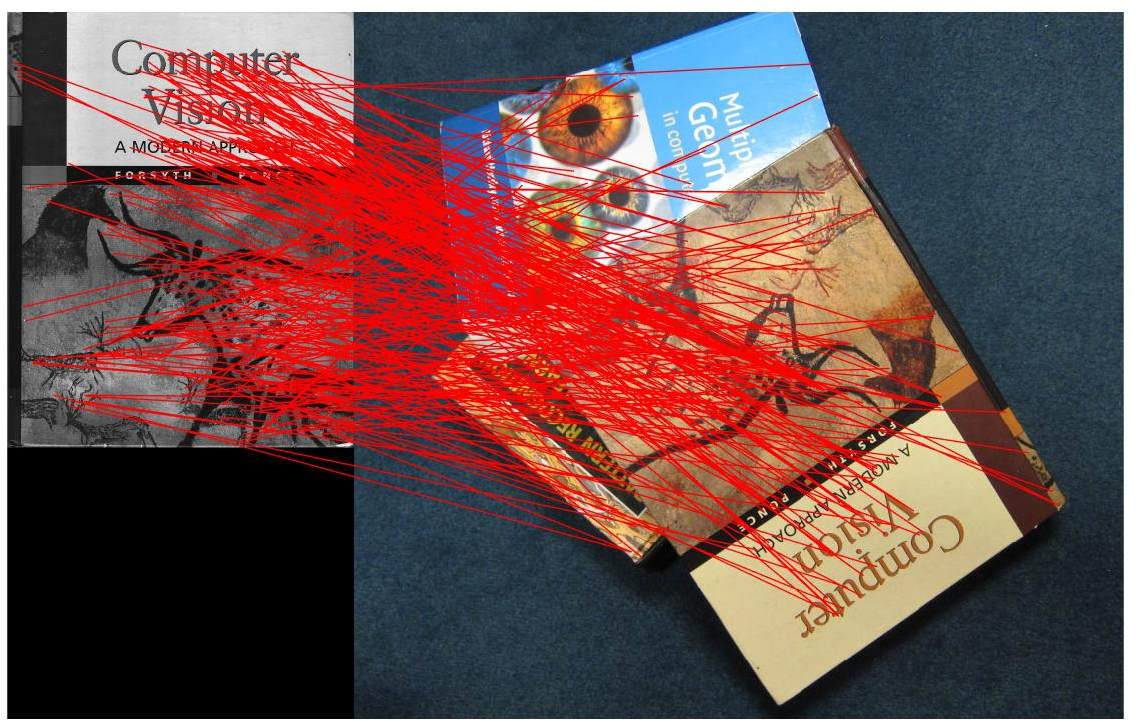
\includegraphics[width=.5\textwidth]{results/BRIEF_pfscan_pile.jpg}} &
        \subfloat[]{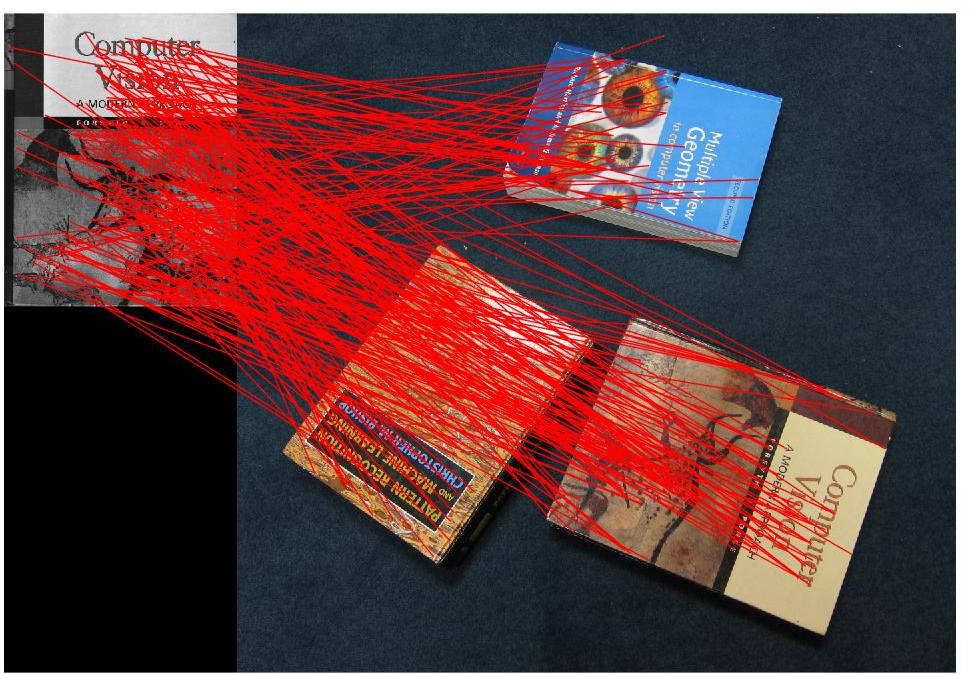
\includegraphics[width=.5\textwidth]{results/BRIEF_pfscan_floor_rot.jpg}} 
    \end{tabular}
\end{figure}
\section*{Q 2.5}
As noted above, BRIEF performs notably worse when forced to match rotated images. I believe this is 
because the BRIEF descriptors are comparisons of pixels in a given area at a fixed orientation. If 
the area underneath the test pattern is rotated, the resulting descriptor changes, often drastically. 

\begin{figure}[H]
\centering
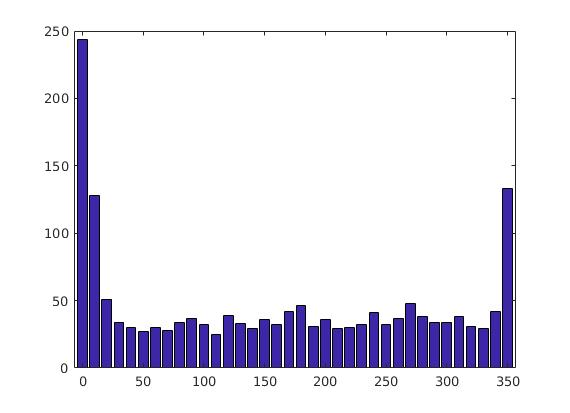
\includegraphics[width=.7\textwidth]{results/brief_rot_test.jpg}
\caption{Bar graph showing count of correct matches between \texttt{model\_chickenbroth.jpg} 
and itself at 10 degree increments.}
\end{figure}
\section*{Q 3}
\subsection*{Q 3.a}
\subsection*{Q 3.b}
There are nine elements in vector $h$. 
\subsection*{Q 3.c}
Four point pairs are required to solve this system, because each point provides two equations.
Because the camera projection matrix only has eight degrees of freedom, we can choose an addiitonal
bound on the matrix without specifying more points. The preferred method is to set the norm
of $H$ to 1.
\subsection*{Q 3.d}
\section*{Q 6.1}
\begin{figure}[H]
\centering
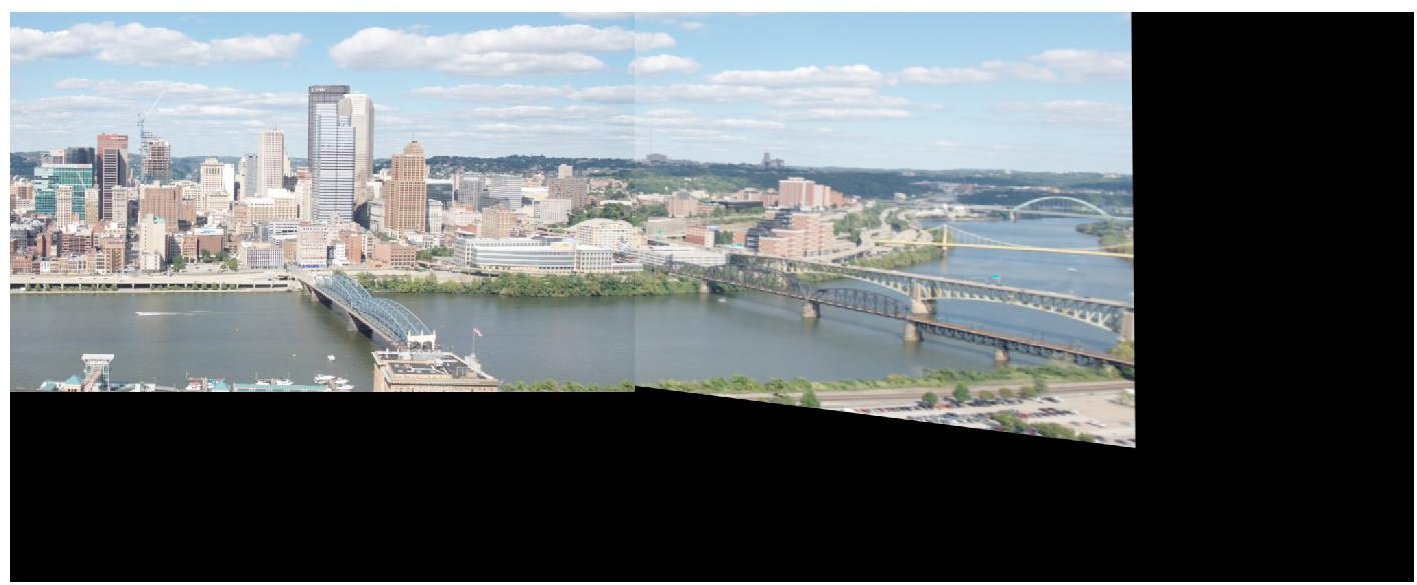
\includegraphics[width=\textwidth]{results/6_1.jpg}
\caption{Initial attempt at panorama creation.}
\end{figure}
\section*{Q 6.3}
\begin{figure}[H]
\centering
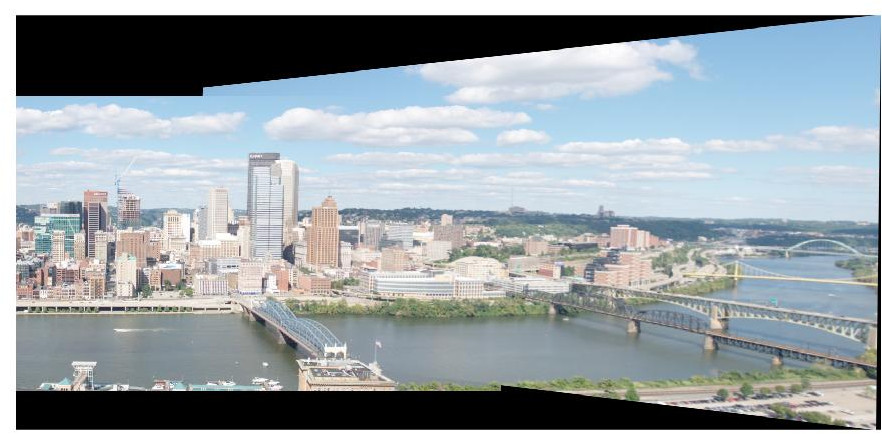
\includegraphics[width=\textwidth]{results/q6_3.jpg}
\caption{Panorama creation after appropriately sizing output images and performing required
translations. The images are already at appropriate scaling after conversion from homogenous 
coordinates.}
\end{figure}

\end{document}
